\newpage
\section{Other useful information}

See also the \textit{The Not So Short Introduction to \LaTeXe}\cite{NotSoShort}
available online at \url{http://tobi.oetiker.ch/lshort/lshort.pdf} or
\url{http://www.ctan.org/tex-archive/info/lshort/english/lshort.pdf}.

\subsection{Example functions}
\begin{align}
F\pa{x} & = \int_{0}^{\infty} \frac{\sqrt{a + x}}{\pa{b + x}^5}~\textrm{d}x
\label{eqn:example}
\end{align}

\subsection{Citing}
When a label is attached to an equation, it can be cited. By adding ``\textbackslash label\{eqn:example\}'' in
the function's \textit{align} environment, it becomes possible to cite equation \eqref{eqn:example} with
``\textbackslash eqref\{eqn:example\}''.

To refence a book, article or other, use \BibTeX. Then cite the document
using its \BibTeX key with ``\textbackslash cite\{BibTeX key\}''. For example,
``\textbackslash cite\{Taflove2005\}'' will give the clickable link \cite{Taflove2005}
which points to the references section.



\subsection{Figures}
Figures should be in PDF or PNG format if compiling using \textbf{pdflatex} or EPS if compiling
with \textbf{latex} (resulting in a DVI file).

Since PDF is a vectorial format, figures in PDF will give higher quality results (if the figure
is in vectorial format that is). Figure \ref{fig:example_figure} shows an example.

\begin{figure}
\begin{center}
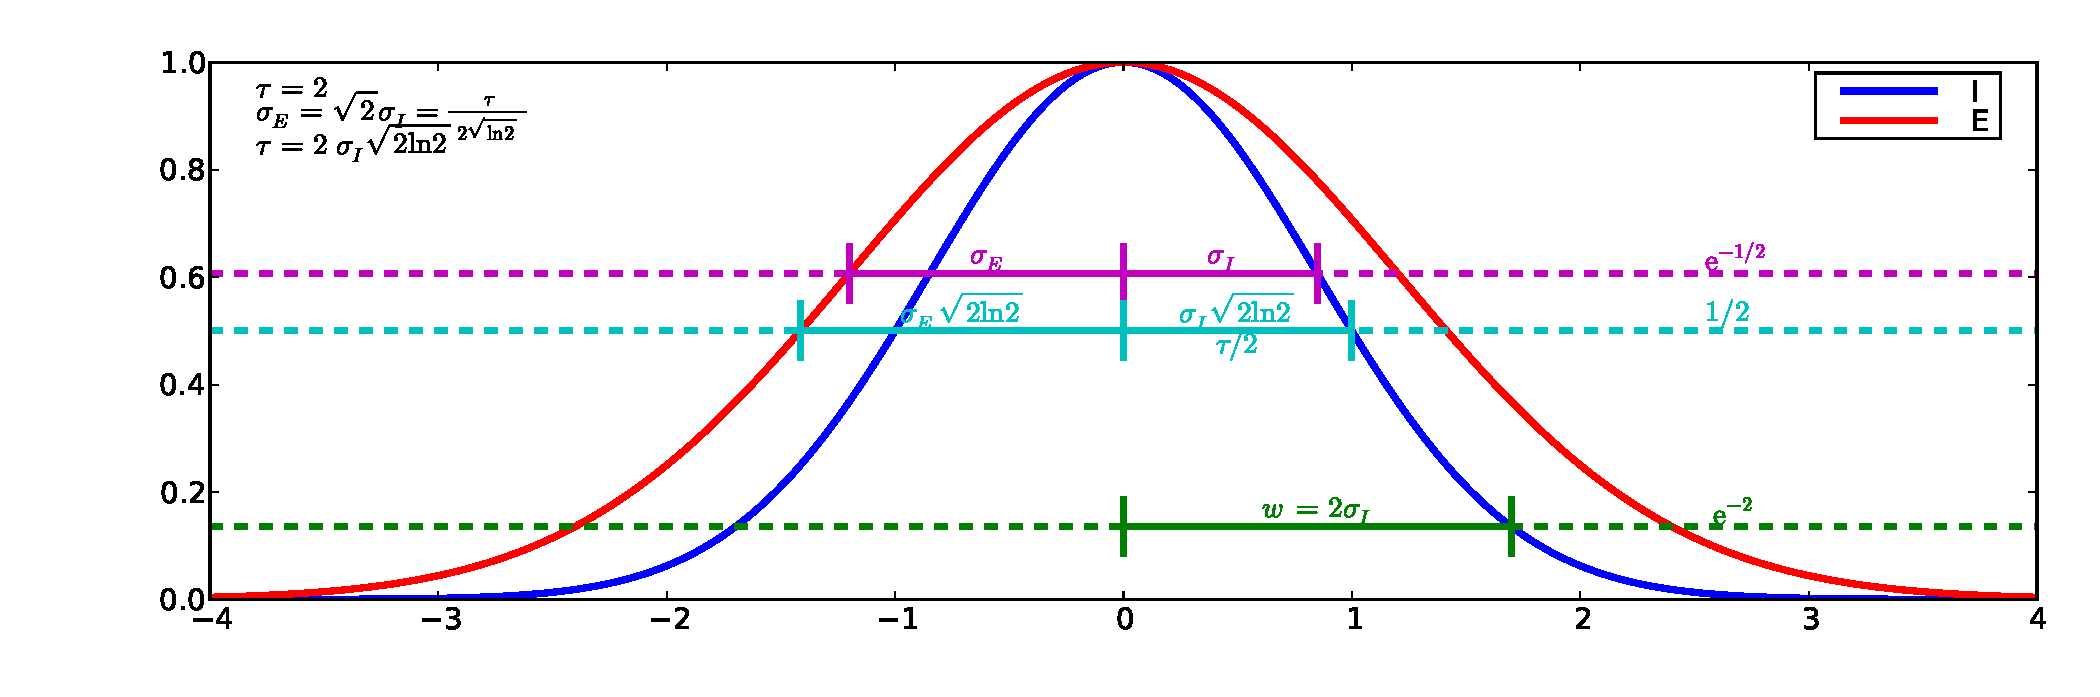
\includegraphics[width=\textwidth]{forme_I_E.pdf}
\end{center}
\caption{This is a caption}
\label{fig:example_figure}
\end{figure}


\subsection{Greek alphabet}

\begin{center}
\begin{tabular}{|l|c||l|c|l|c||l|c|} \hline
Code                        & Result            & Code                        & Result      & Code                        & Result          & Code                        & Result          \\ \hline \hline
\textbackslash alpha        & $\alpha$          & \textbackslash mu           & $\mu$       & \textbackslash chi          & $\chi$          & \textbackslash Sigma        & $\Sigma$        \\ \hline
\textbackslash beta         & $\beta$           & \textbackslash nu           & $\nu$       & \textbackslash psi          & $\psi$          & \textbackslash varSigma     & $\varSigma$     \\ \hline
\textbackslash gamma        & $\gamma$          & \textbackslash xi           & $\xi$       & \textbackslash omega        & $\omega$        & \textbackslash Upsilon      & $\Upsilon$      \\ \hline
\textbackslash delta        & $\delta$          & \textbackslash pi           & $\pi$       & \textbackslash Gamma        & $\Gamma$        & \textbackslash varUpsilon   & $\varUpsilon$   \\ \hline
\textbackslash epsilon      & $\epsilon$        & \textbackslash varpi        & $\varpi$    & \textbackslash varDelta     & $\varDelta$     & \textbackslash Phi          & $\Phi$          \\ \hline
\textbackslash varepsilon   & $\varepsilon$     & \textbackslash rho          & $\rho$      & \textbackslash Theta        & $\Theta$        & \textbackslash varPhi       & $\varPhi$       \\ \hline
\textbackslash zeta         & $\zeta$           & \textbackslash varrho       & $\varrho$   & \textbackslash varTheta     & $\varTheta$     & \textbackslash Psi          & $\Psi$          \\ \hline
\textbackslash eta          & $\eta$            & \textbackslash sigma        & $\sigma$    & \textbackslash Lambda       & $\Lambda$       & \textbackslash varPsi       & $\varPsi$       \\ \hline
\textbackslash theta        & $\theta$          & \textbackslash varsigma     & $\varsigma$ & \textbackslash varLambda    & $\varLambda$    & \textbackslash Omega        & $\Omega$        \\ \hline
\textbackslash vartheta     & $\vartheta$       & \textbackslash tau          & $\tau$      & \textbackslash Xi           & $\Xi$           & \textbackslash varOmega     & $\varOmega$     \\ \hline
\textbackslash iota         & $\iota$           & \textbackslash upsilon      & $\upsilon$  & \textbackslash varXi        & $\varXi$        &                             &                 \\ \hline
\textbackslash kappa        & $\kappa$          & \textbackslash phi          & $\phi$      & \textbackslash Pi           & $\Pi$           &                             &                 \\ \hline
\textbackslash lambda       & $\lambda$         & \textbackslash varphi       & $\varphi$   & \textbackslash varPi        & $\varPi$        &                             &                 \\ \hline
\end{tabular}
\end{center}

